\documentclass{article}

% WM-PAI @ NeurIPS 2026 workshop version (non-archival, double-blind).
% ~4 pages body + references; NeurIPS 2026 template, submission mode.
% Full archival version targeted at ICLR 2027.
\usepackage{neurips_2026}

\usepackage[utf8]{inputenc}
\usepackage[T1]{fontenc}
\usepackage{hyperref}
\usepackage{url}
\usepackage{booktabs}
\usepackage{amsfonts,amsmath}
\usepackage{nicefrac}
\usepackage{microtype}
\usepackage{xcolor}
\usepackage{graphicx}

% =====================================================================
% NUMBER MACROS — single source of truth (verified manifest, 2026-09-06).
% \pendingnum renders a visible red marker so no placeholder can silently
% survive into the submitted PDF.
\newcommand{\pendingnum}[1]{\textcolor{red}{\textbf{[#1]}}}
% Frozen anchors:
\newcommand{\TRLanchorRepro}{0.1934}  % our re-evaluation of the official ckpt
\newcommand{\TRLanchorPub}{0.1956}    % published CNextU-net one-step test VRMSE
\newcommand{\TRLwindows}{873}         % official test windows (paired stats)
% Round 1 — one-step objective, 3 seeds:
\newcommand{\TRLvanilla}{$0.19307 \pm 0.00007$}
\newcommand{\TRLquantum}{$0.19315 \pm 0.00007$}
\newcommand{\TRLmlp}{$0.19314 \pm 0.00016$}
\newcommand{\TRLpvalue}{$\le 1.9{\times}10^{-2}$ per seed (best $6{\times}10^{-12}$)}
\newcommand{\TRLwinrate}{52.5--60.1\%}
% Round 2 — TD objective (k=4), 3 seeds, window 13:30:
\newcommand{\TDvanilla}{$1.0301 \pm 0.0449$}
\newcommand{\TDquantum}{$\mathbf{0.9528 \pm 0.0542}$}
\newcommand{\TDmlp}{$1.0322 \pm 0.0259$}
\newcommand{\TDpvalue}{seed-level 3/3; per-traj.\ ($n{=}9$) 1/3 Holm-sig.\ vs MLP, 0/3 vs vanilla}
\newcommand{\TDwinrate}{3/3 seeds below anchor}
% Qubit ladder (sprint arena, fixed 2,000 steps, TD k=4, 3 seeds, VRMSE@8):
\newcommand{\QLzero}{$0.9567 \pm 0.2554$}    % FNO trunk alone, 0 qubits
\newcommand{\QLfive}{$0.8427 \pm 0.0709$}     % 1x5q register
\newcommand{\QLten}{$0.9332 \pm 0.2166$}      % 1x10q register
\newcommand{\QLtwenty}{$0.9269 \pm 0.2792$}   % 2x10q registers
\newcommand{\QLthirty}{$0.8447 \pm 0.0511$}  % 30q Rydberg 3x10
\newcommand{\QLmlp}{$0.9534 \pm 0.1354$}     % matched-MLP 30d control
\newcommand{\QLgeo}{$0.8951 \pm 0.1367$}     % conditioned-geometry 30q
\newcommand{\MHDmlp}{0.1770--0.1771}          % s1337 arms, final/best val
\newcommand{\ScalingEq}{$\mathrm{VRMSE@8}(n) = 0.849 + 0.108\, e^{-n/n^\star}$
with fitted $n^\star \approx 0.1 \ll 5$: saturation below the smallest tested
register, and a constant fits the $n \ge 5$ points equally well}
% Verdict macros:
\newcommand{\AblationVerdict}{In the pre-registered training-side ablation,
retraining the identical adapter with blockade interactions zeroed ---
product state from step 0, same TD protocol, three seeds --- loses the
effect: 13:30 test VRMSE $1.0156 \pm 0.0433$ with only 1/3 seeds below the
anchor (vs 3/3 entangled), and the entangled arm's rollout-validation
selection is better on every seed (0.5783/0.5771/0.5642 vs
0.5923/0.5807/0.5739). Zeroing $V_{ij}$ removes entanglement \emph{and}
the mean-field nonlinearity of the interaction term, so the licensed
conclusion is that the blockade interactions appear dispensable at
inference yet necessary during optimization in this regime; separating entanglement from mean-field interaction requires a
Gutzwiller-type control (interactions kept, entanglement forbidden). A
pre-registered mean-field pilot in the arena --- a product state by
construction --- matches the entangled register on all three seeds
(VRMSE@8 $0.839 \pm 0.046$ vs $0.845 \pm 0.051$; 0.891/0.825/0.802 vs
0.903/0.826/0.806), pointing to the interaction nonlinearity rather than
entanglement; the decisive official-protocol arms complete after
submission. The gain tracks training \emph{through} interacting
Rydberg dynamics rather than a generic high-dimensional bottleneck.}
% =====================================================================

\title{QUOTA: A Few Configurable Qubits Improve\\
Long-Horizon Rollouts of Physical World Models}

\author{Anonymous}

\begin{document}

\maketitle

\begin{abstract}
World models degrade past the spatial-mean floor over long rollouts, even
at foundation scale \citep{ohana2024thewell,mccabe2025walrus}. We
hypothesize that the failure sits in the analog part of the signal:
physical fields separate into an easily digitized component and a
continuous analog component \citep{mallat1989multiresolution,daubechies1992ten},
so assigning only the analog part to a small configurable quantum register
should recover long-horizon accuracy with today's qubit counts. QUOTA
(\emph{QUantum Offload of The Analog core}) implements this as one
parametrized world model: a Rydberg register whose per-qubit detunings are
conditioned on the input state and whose geometry is an optimized
blockade-coupling graph, inside a pretrained classical model that carries
the rest. Under a pre-registered protocol with parameter- and tuning-matched
controls and kill rules on The Well, the register drops into the official
CNextU-net checkpoint without harm and, trained through rollouts, is the
only arm that improves the hardest long-horizon window on every seed (test VRMSE \TDquantum{}, 7.5--7.7\% lower than vanilla fine-tuning \TDvanilla{} and a matched MLP \TDmlp{}; directional at nine trajectories). The trained register is inference-inert
yet depends on its interactions during training, accuracy is flat from
five qubits upward, and a 3-D MHD grid (three arms, three seeds) is a null; a
ten-benchmark industrial ladder spanning fusion, fission proxies,
geothermal heat exchange, and video physics extends the protocol. Thirty
simulated qubits are classically simulable
\citep{schuld2022advantage,cerezo2025barren}: the claim is inductive bias
on the hardware that exists, not quantum advantage.
\end{abstract}

\section{Introduction}
\label{sec:intro}

World models --- learned simulators that roll a latent state forward under
dynamics --- increasingly serve as the interface between machine learning
and physics \citep{ohana2024thewell,mccabe2025walrus,gao2026lingbotworld}.
Their central unsolved failure is \emph{physical consistency over long
horizons}: on The Well, the best official baseline (CNextU-net) reaches
one-step test VRMSE \TRLanchorPub{} on
\texttt{turbulent\_radiative\_layer\_2D} (TRL2D) but degrades to 1.01 by
rollout window 13:30 --- worse than predicting the spatial mean --- and even
the 1.3B foundation model Walrus exceeds this floor at long horizon
\citep{ohana2024thewell,mccabe2025walrus}.

Two literatures make claims that bear on this failure. First, \emph{analog
quantum simulation}: neutral-atom platforms natively evolve Rydberg
Hamiltonians, with inputs encoded directly into detunings, positions, and
drives of up to 108 qubits \citep{kornjaca2024aquila}, and Hamiltonian input
encoding is provably expressive \citep{xia2026magicqrc}. Second,
\emph{quantum modules for foundation models}: unitary and quantum(-inspired)
adapters fine-tune frozen large models at extreme parameter efficiency
\citep{koikeakino2025quantumpeft,raj2025quic,aizpurua2026cayley,zhao2026mqadapter}.
To our knowledge, neither literature has produced a matched-control win
on a public physical-simulation benchmark: quantum-informed priors report turbulence rollout gains, but as offline regularizers against over-parameterized classical priors, with an advantage claim
\citep{wang2026qiml,xue2026qcml}; the closest in-model attempt, a 5-qubit
mixer in a 3D FNO surrogate on proprietary laser-processing data, beat a
larger dense-mixer FNO on mean-error metrics but was matched or beaten by
its own parameter-matched MLP-mixer control on all but one metric
\citep{papierz2026hqlpfno}; and reservoir studies show apparent quantum
edges evaporating under equal-tuning classical baselines
\citep{pandey2026qrcbaselines}. Concurrent theory proves that certain classical environments with
long-range (irrational-phase) memory admit an exact single-qutrit quantum
world model while every finite classical model misaligns the optimal policy
\citep{lumbreras2026irreducible}; a fully observed finite-difference PDE is
Markov in its state and lies outside that construction, so our contribution
is empirical and control-matched. The similarly named QSWM
\citep{sun2026qswm} is quantum-inspired (no register) and, against matched
controls on cellular automata, finds its edge confined to short horizons
--- the opposite profile of ours.

Our premise connects the two claims. Analog quantum hardware may be the
natural substrate for physical dynamics, but no practical application fits
on today's qubit counts whole --- and real simulations are rarely uniformly
quantum-hard: they mix classically easy, effectively discrete structure with
a harder analog core. Signal analysis offers the analogy: Fourier and multiresolution
decompositions separate a field into sparse, effectively discrete
structure and continuous spectral content
\citep{mallat1989multiresolution,daubechies1992ten}, which neural operators
already exploit classically \citep{li2021fno} (an analogy, not a hardness claim). We therefore adopt the division-of-labor stance that quantum-informed
workflows \citep{wang2026qprior} and modular frozen-block designs
\citep{qi2026lego} also articulate, but instantiate it in the model rather
than in the loss: the qubit budget is a scarce resource to be
\emph{allocated}: a reconfigurable, input-parameterized
register is steered toward the highest-complexity analog subprocess of the
problem at hand, while a pretrained classical world model carries the rest
(in the experiments below the classical trunk is co-fine-tuned; the
strictly frozen-backbone setting is the archival extension). If the
division of labor is right, small fixed budgets become useful on current
hardware, and rollout accuracy versus qubit count --- ``fidelity''
throughout means rollout accuracy, not quantum state fidelity --- becomes a
measurable scaling question rather than a wait for million-qubit machines.
The premise is a motivating conjecture: no experiment below identifies or
steers the register toward a particular subprocess (it reads a pooled
latent), and the alternative that the register acts as an
$n$-independent training perturbation is kept in view. This is the
hypothesis our protocol is built to test --- and, if warranted, kill.

Contributions:
\begin{enumerate}
  \item \textbf{Checkpoint surgery against a published number.} We insert
  the bottleneck at the neck of the \emph{official released} CNextU-net
  checkpoint from The Well and fine-tune, targeting its published
  \TRLanchorPub{} one-step test VRMSE \citep{ohana2024thewell} with paired
  per-window Wilcoxon significance over the \TRLwindows{} official test
  windows --- the methodology (official-checkpoint surgery +
  published-number target + paired statistics) and its result are the
  contribution, not the architecture
  \citep{ma2025qufex,liu2026hqfnet,ali2026phqfno}.
  \item \textbf{An input-conditioned analog ansatz with reconfigurable
  structure.} Data-dependent detunings, gradient-trained 2D atom geometry,
  and global drive parameterize the Rydberg generator via exact statevector
  autodiff; the trained object lies in the native Rydberg Hamiltonian
  family, while mapping it onto device constraints (sign and static-pattern
  limits of local detuning on current machines) is future work. ReCon co-trains positions, site couplings, and drive derivative-free at
four atoms \citep{silver2024recon}, ResQ feeds inputs into per-atom
detunings on fixed lattices \citep{chen2026resq}, and PulserDiff
differentiates pulses and positions as tooling \citep{pulserdiff2025};
position gradients were argued ineffective under the divergent $r^{-6}$
term \citep{dekeijzer2025consensus}, which we bound by clamping distances.
To our knowledge no prior work composes a learned detuning map with
autodiff-trained geometry as a layer of a predictive model
  (\S\ref{sec:system}).
  \item \textbf{A pre-registered, kill-rule protocol.} Qubit-count sweeps exist in looser, non-parameter-matched forms
\citep{ionq2026scaling,kornjaca2024aquila,vyskubov2026scaling,zabihi2026hqpinn},
and controlled quantum-sidecar insertions with matched bottleneck controls
exist for classification \citep{levy2026sidecar}; we contribute, to our
knowledge, the first \emph{pre-registered, tuning-and-parameter-matched,
kill-ruled} instantiation on a public PDE benchmark (significance-tested in
the TRL2D campaign, \S\ref{sec:campaign}): matched
  MLP/product-state controls \citep{pandey2026qrcbaselines,bowles2024better},
  explicit kill rules (if controls match, the negative result is the paper),
  and a dequantization suite, under the honest-framing standard of
  \citet{schuld2022advantage} and the classical-simulability caveat of
  \citet{cerezo2025barren}.
  \item \textbf{A fidelity-versus-qubit-count scaling measurement.} Holding
  total parameters, data, and step budget fixed, we sweep the register size
  $n \in \{0,5,10,20,30\}$ and report rollout accuracy as a function of
  $n$, finding it flat within seed noise for $n \ge 5$
  (\S\ref{sec:scaling}).
\end{enumerate}

\section{System}
\label{sec:system}

A classical trunk produces a latent field $z$; an attention pool yields
$h \in \mathbb{R}^d$; a linear map sets per-qubit, per-layer detunings
$\delta = \pi \tanh(W h)$; each 10-qubit register evolves under
\begin{equation*}
H_{\mathrm{Ryd}}/\hbar = \sum_i \tfrac{\Omega_\ell}{2} X_i - \sum_i
\delta_{\ell,i} n_i + \sum_{i<j} \frac{C_6}{|r_i - r_j|^{6}}\, n_i n_j
\end{equation*}
with trainable times $\tau_\ell$, global drives $\Omega_\ell$, and trainable
atom coordinates $r_i$ (geometry-as-parameter); $\langle Z_i \rangle$
readouts re-enter the trunk through a zero-initialized gated residual.

\paragraph{Instantiation.} $n_i = |r\rangle\langle r|_i$ is the Rydberg
projector on atom $i$. The evolution is a first-order digital--analog split
of $H_{\mathrm{Ryd}}$ with $L{=}4$ layers: layer $\ell$ applies, per
qubit, the conditioned detuning phase $R_z(\delta_{\ell,i})$ fused with the
global drive $R_x(\Omega_\ell)$, then the diagonal interaction phase
$\exp(-i\tau_\ell \sum_{i<j} V_{ij} n_i n_j)$ with
$V_{ij} = C_6/|r_i - r_j|^6$, $C_6 = 1$ in blockade-radius units and
distances clamped at $0.5\,R_b$. Detunings are
$\delta_{\ell,i} = b_{\ell,i} + \pi\tanh(W_\ell h)$ with $W$ zero-initialized;
$\Omega_\ell$ and $\tau_\ell$ are initialized at 0.5 and 0.3; positions
start on a unit lattice with $\sigma{=}0.05\,R_b$ jitter; readout is
$\langle Z_i\rangle$. The block is inserted at the CNextU-net neck
($d{=}672$). Each register has 108 Hamiltonian parameters ($b$, $r$,
$\Omega$, $\tau$) plus the conditioning map $W$ of $80 \times d$ entries
($\approx$2k at $d{=}24$ in the arena, 53.8k at the neck); 30 simulated
qubits are three \emph{mutually non-interacting} 10-qubit registers
(inter-register $C_6$ omitted; entanglement is intra-register
\citep{huang2020patchgan}). Every baseline
implements the identical pool$\to$core$\to$residual interface at matched
total parameters (within 0.4\% among adapter-bearing arms; the bare trunk
sits 0.5\% below). Each register trains with a batched complex64
\emph{exact} statevector propagator with autograd gradients, cross-checked
against CUDA-Q statevector simulation to $\max_i |\Delta\langle Z_i\rangle|
\le 10^{-6}$.

The register is thus \emph{reconfigurable and input-conditioned}: detunings
are functions of the simulation state, and geometry-as-parameter is a
natively realizable knob of the platform --- optical tweezers assemble atoms
into user-defined 2D/3D arrangements at the $\sim$100-atom scale
\citep{barredo2018synthetic}, and coherent arrays now reach 6{,}100 atoms
\citep{manetsch2025tweezer}; the same Hamiltonian family also supports
annealing-style schedules \citep{ebadi2022quantum}.

\paragraph{Configuring the register.} Register configuration is itself a
search over parameterized geometric graphs. In this study the configuration
is gradient-trained end-to-end and, in one variant, input-conditioned
(Table~\ref{tab:ladder}); a smoke-scale gradient-free search (CMA-ES, $\sim$200 evaluations per
regime; best VRMSE@8 1.14--1.31) was not competitive with gradient
training. Figure~\ref{fig:registers} shows the learned configurations: a small
coherent lattice contraction, with per-input adaptation carried by
low-rank detuning modes rather than atom relocation.


\begin{figure}[t]
\centering
\IfFileExists{fig_registers.pdf}{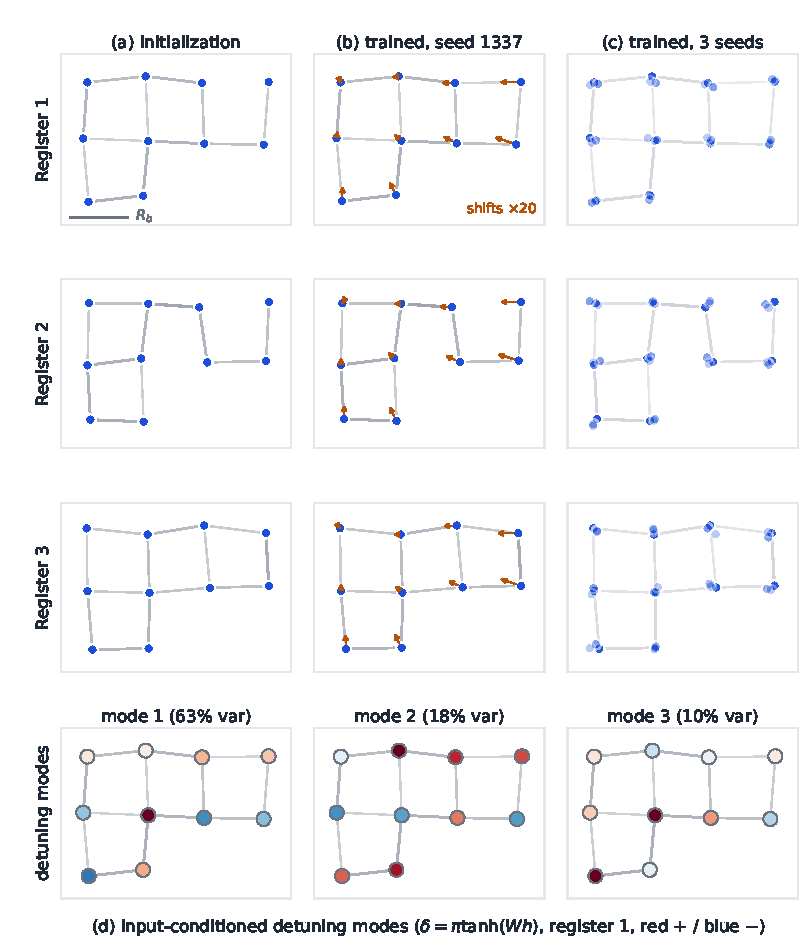
\includegraphics[width=0.5\linewidth]{fig_registers.pdf}}{}
\caption{\small Register configurations (three blockade-decoupled 10-atom Rydberg
registers, trainable 2D geometry, blockade-radius units; edges: pairs with
$C_6/r^6$ at least half the coupling at $R_b$, thicker $=$ stronger).
\emph{(a)}~Initialization (lattice $+\ \sigma{=}0.05\,R_b$ jitter,
re-derived from the training seed). \emph{(b)}~TD-trained geometry (seed
1337), displacements $\times 20$: a small coherent contraction (mean radial
shift $-0.007\,R_b$, all registers and seeds) that strengthens couplings and
preserves topology. \emph{(c)}~Three seeds agree to $\le 0.11\,R_b$ rms.
\emph{(d)}~Per-input reconfiguration via detunings $\delta=\pi\tanh(Wh)$:
the top three singular modes of the conditioning map hold 91\% of its
variance; the dominant mode is shared across registers
($|v_1^{(1)}\!\cdot v_1^{(2)}|=0.80$).}
\label{fig:registers}
\end{figure}

\section{Protocol}
\label{sec:protocol}

\paragraph{Task and metric.} Given a history $(x_{t-3},\dots,x_t)$ of field
snapshots $x_t \in \mathbb{R}^{C \times H \times W}$, predict $x_{t+1}$;
long-horizon behavior is evaluated by autoregressive rollout; The Well's
official rollout scores average VRMSE over step windows 6--12 and 13--30
(denoted 6:12 and 13:30). The official
metric is variance-scaled RMSE,
$\mathrm{VRMSE} = \|\hat x - x\|_2 / \sqrt{\|x - \bar x\|_2^2 + \epsilon}$ ($\epsilon = 10^{-7}$; computed per
channel and averaged over channels and windows, following The Well's
reference implementation), with $\mathrm{VRMSE}=1$ equivalent to
predicting the spatial mean \citep{ohana2024thewell}. Throughout,
$\pm$ denotes the standard deviation across three seeds.

\paragraph{Hypothesis and kill rule.} H1: a quantum bottleneck with
input-conditioned Rydberg dynamics improves rollout accuracy over parameter-
and tuning-matched classical controls. Kill rule (pre-registered): if the
matched control is statistically indistinguishable from or better than the
quantum variant across seeds, the hypothesis is reported dead in this
regime.
Primary goal: one-step test VRMSE $< \TRLanchorPub$ on TRL2D, significant
under a paired per-window Wilcoxon test over the \TRLwindows{} official
test windows against the official CNextU-net checkpoint (one-sided,
ours $<$ anchor; Holm-corrected across the three seeds; windows overlap
within trajectories, so per-window $p$-values are anti-conservative and are
always read together with seed-level consistency). As anchor we
re-evaluated the official checkpoint with our pipeline: mean VRMSE
\textbf{\TRLanchorRepro} over \TRLwindows{} windows (published:
\TRLanchorPub; 1.1\% discrepancy) --- we adopt the stricter reproduced
number as the bar. Hypotheses, kill rules, and ablations were timestamped
in the project repository before the corresponding runs (commit hashes
released with the code; self-timestamping is weaker than an external
registry). Registration was \emph{sequential}: the one-step endpoint was
the original primary; the Round-2 TD protocol --- window 13:30,
best-checkpoint selection by rollout-validation VRMSE@8, seed-paired
comparison against both controls --- was specified after Round 1's null
was known and fixed before any Round-2 run, so it is confirmatory within
its round and sequentially registered relative to the original plan; the
interaction ablation and the $\{5,10,20\}$q ladder arms were likewise
fixed before execution (after the 0q/30q arena runs).

\section{Results}
\label{sec:results}

\subsection{Official benchmark (TRL2D): one-step null, rollout win}
\label{sec:campaign}

The campaign fine-tunes the official released CNextU-net checkpoint under
the official protocol, three arms (vanilla continued / matched-MLP control /
30q Rydberg) $\times$ three seeds, single-shot test evaluation per
best-on-validation model (Round 1: one-step validation VRMSE; Round 2:
rollout-validation VRMSE@8, the eighth-step error of an 8-step validation
rollout), paired per-window Wilcoxon against the reproduced anchor
(Table~\ref{tab:campaign}). \textbf{Round 1 (one-step objective):}
the quantum arm beats the anchor significantly (\TRLquantum{} vs
\TRLanchorRepro; win rate \TRLwinrate, $p$ \TRLpvalue) --- but vanilla
fine-tuning matches it (\TRLvanilla). All arms improve minutely and
indistinguishably: the pre-registered kill rule fired, and we report the
attribution null. \textbf{Round 2 (temporal-difference/pushforward
objective \citep{brandstetter2022message}: the model is unrolled $k{=}4$
autoregressive steps on its own predictions and the loss is applied at the
last step, with gradients through that step only),}
evaluated on the official test rollout windows (published CNextU-net
0.54 / 1.01 at windows 6:12 / 13:30; our anchor reproduction
0.5482 / 1.0132): the quantum arm is the only configuration that improves
the long-horizon window on every seed --- 13:30 VRMSE \TDquantum{} vs
vanilla \TDvanilla{} and matched-MLP \TDmlp{} --- winning the seed-paired
comparison 3/3 against both controls while matching them on the medium
window (6:12: quantum 0.5278, vanilla 0.5216, MLP 0.5271, anchor 0.5482).
At the trajectory level the test set is small ($n{=}9$ test
trajectories), and paired per-trajectory Wilcoxon tests on window 13:30
are correspondingly underpowered: the quantum arm beats vanilla on 6/9,
7/9, and 7/9 trajectories across seeds (one-sided $p = 0.21, 0.037,
0.027$; none survives Holm), beats the matched MLP on 5/9, 6/9, 7/9
($p = 0.50, 0.21, 0.0098$; the last survives Holm), and beats the anchor
on 4/9, 5/9, 6/9 ($p = 0.54, 0.33, 0.065$) --- so the seed-mean
improvement is carried by a subset of trajectories. This Round-2 evidence
is therefore directional seed-level consistency, not trajectory-level
significance under the pre-registered standard. TD arms are rollout models: their one-step test error rises by
design (to 0.31--0.33 across all three arms, vs 0.193 for the one-step
arms); Figure~\ref{fig:training} (left) shows the fine-tuning
trajectories ---
arms overlap step-by-step and separate at best-checkpoint selection,
consistent with the seed-level framing. Figure~\ref{fig:fields} visualizes
a full rollout: prediction error is an \emph{interface} phenomenon,
concentrated where the density gradient is largest, and the quantum arm is
the best of the TD arms at tracking the front's position.

\begin{table}[t]
\centering
\footnotesize
\setlength{\tabcolsep}{3pt}
\resizebox{\linewidth}{!}{%
\begin{tabular}{llccc}
\toprule
Round & Arm & Test VRMSE (3 seeds) & significance vs anchor & win rate \\
\midrule
--- & official checkpoint (anchor) & \TRLanchorRepro{} / 1.0132 & --- & --- \\
\midrule
1 (one-step) & vanilla continued & \TRLvanilla & 3/3 seeds $p<0.05$ & --- \\
1 (one-step) & $+$ matched MLP (control) & \TRLmlp & 2/3 seeds $p<0.05$ & --- \\
1 (one-step) & $+$ 30q Rydberg & \TRLquantum & 3/3 seeds (best $6{\times}10^{-12}$) & \TRLwinrate \\
\midrule
2 (TD), 13:30 & vanilla continued & \TDvanilla & --- & --- \\
2 (TD), 13:30 & $+$ matched MLP (control) & \TDmlp & --- & --- \\
2 (TD), 13:30 & $+$ 30q Rydberg & \TDquantum & \TDpvalue & \TDwinrate \\
\bottomrule
\end{tabular}}
\vspace{2pt}
\caption{\small TRL2D official-protocol campaign. Round 1: one-step test
mean-VRMSE (anchor \TRLanchorRepro); kill rule fired --- attribution null.
Round 2: rollout window 13:30 test VRMSE (anchor 1.0132, published 1.01);
the quantum arm is the only one below the anchor on 3/3 seeds and beats
both controls seed-paired 3/3; per-trajectory Wilcoxon tests ($n{=}9$)
are underpowered and reach Holm-corrected significance only vs the MLP on
one seed (\S\ref{sec:campaign}).}
\label{tab:campaign}
\end{table}

\begin{figure}[t]
\centering
\IfFileExists{fig_training.pdf}{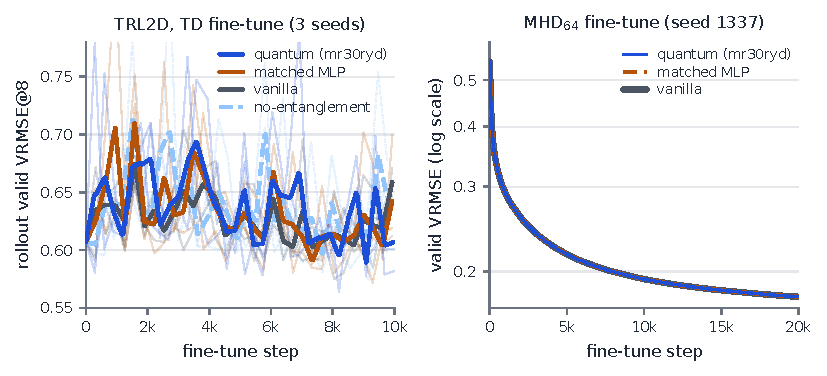
\includegraphics[width=0.72\linewidth]{fig_training.pdf}}{}
\caption{\small Fine-tuning dynamics. \emph{Left:} TRL2D TD fine-tuning from the
official checkpoint (thin: individual seeds; bold: 3-seed mean of the
rollout-validation selection metric). Best-checkpoint selection values are
quantum 0.564--0.578 across seeds vs vanilla 0.575--0.591, matched-MLP
0.572--0.580, and no-entanglement 0.574--0.592: the arms overlap
step-by-step and separate at best-checkpoint selection, matching the
directional seed-level evidence of Table~\ref{tab:campaign}.
\emph{Right:} \texttt{MHD\_64} fine-tuning (seed 1337, log scale); all
three arms converge indistinguishably to validation VRMSE $\approx$0.177.}
\label{fig:training}
\end{figure}

\subsection{Qubit-count scaling}
\label{sec:scaling}

The premise predicts that, at fixed total parameters and budget, rollout
fidelity should improve as the analog register grows. We measure this in an
internal fixed-budget \emph{sprint arena} (a 3-regime TRL2D subset, fixed
2{,}000 steps, TD $k{=}4$, 3 seeds; the metric, VRMSE@8, is the VRMSE of
the eighth autoregressive rollout step averaged over strided starts;
$\sim$1.33M total parameters, matched within
0.4\% across variants; internally comparable, \emph{not} comparable to the
official table). The training objective interacts strongly with the
register: switching from one-step to TD training improves the quantum
variant by 23\% ($1.1002 \pm 0.1939 \to$ \QLthirty), the classical
control by 10\% ($1.0574 \pm 0.0574 \to$ \QLmlp), and the bare trunk by
under 1\% ($0.9637 \pm 0.0048 \to$ \QLzero) --- in this arena, adapters
only show their edge under rollout-aware training. Under TD, the 30-qubit
Rydberg bottleneck beats the matched-MLP control on 3/3 seeds
(0.903/0.826/0.806 vs 1.098/0.933/0.829) with the best mean and lowest
variance; an input-conditioned-geometry variant reaches \QLgeo{} ---
worse than the static-layout register, consistent with adaptation being
carried by detunings on this task.
Table~\ref{tab:ladder} and Figure~\ref{fig:scaling} report the completed
ladder. The measured answer is \emph{immediate saturation}: the five-qubit
register already reaches the 30-qubit level (\QLfive{} vs \QLthirty),
intermediate counts are statistically indistinguishable within seed noise
(10q \QLten; 20q \QLtwenty), and the three-constant saturating fit
degenerates to a step at the smallest tested register --- \ScalingEq.
Given the 0-qubit arm's seed variance (the 5-qubit register is better on
2/3 seeds), even the step is at the edge of resolution: the ladder
\emph{bounds} where the curve could rise rather than establishing a law.
Two readings are compatible with a flat curve: that this arena's analog
core is small enough for five qubits (the premise's reading), or that the register acts as an $n$-independent perturbation of TD
training --- the reading a frozen-block bound predicts \citep{qi2026lego}. One datum
separates them only weakly: the 30-dimensional matched MLP
(\QLmlp) does not reach what five qubits reach (\QLfive), so the
\emph{structure} of the bottleneck rather than its width appears to
matter --- suggestive at three seeds, not conclusive.

\begin{table}[t]
\centering
\small
\begin{tabular}{lcc}
\toprule
Register (fixed total params) & Qubits & VRMSE@8 (3 seeds) \\
\midrule
FNO trunk alone & 0 & \QLzero \\
$+$ Rydberg register & 5 & \QLfive \\
$+$ Rydberg register & 10 & \QLten \\
$+$ Rydberg registers & 20 & \QLtwenty \\
$+$ Rydberg registers ($3{\times}10$) & 30 & \QLthirty \\
\midrule
$+$ matched MLP 30-dim (control) & --- & \QLmlp \\
$+$ 30q, conditioned geometry & 30 & \QLgeo \\
\bottomrule
\end{tabular}
\vspace{2pt}
\caption{\small Rollout accuracy versus qubit count (internal sprint arena, fixed
budget, 3 seeds; $\pm$ = sample SD). The 0q and 30q arms ran first (arena
study); the interior $\{5,10,20\}$q arms were pre-registered before
execution and completed before submission. Points above 10 qubits add
registers of 10, not larger registers. The curve is flat within seed
noise for $n \ge 5$: the ladder bounds, not resolves, any rise
(\ScalingEq).}
\label{tab:ladder}
\end{table}

\begin{figure}[t]
\centering
\IfFileExists{fig_scaling.pdf}{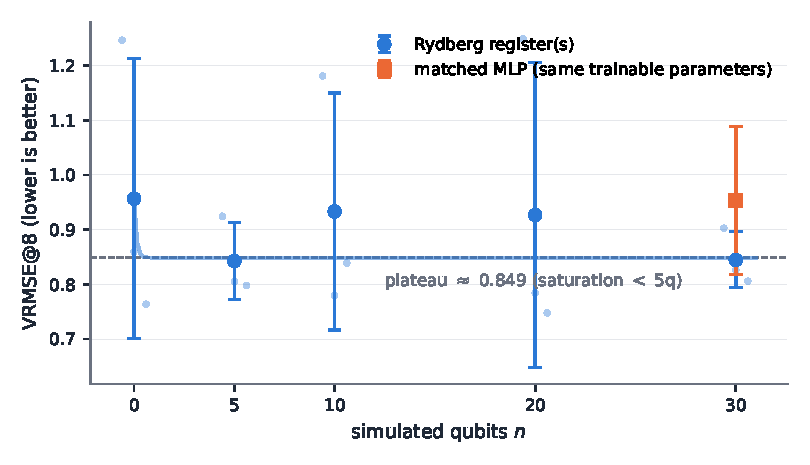
\includegraphics[width=0.64\linewidth]{fig_scaling.pdf}}{\fbox{\parbox{0.9\linewidth}{\centering\pendingnum{fig\_scaling.pdf missing from bundle}}}}
\caption{\small Rollout error versus qubit count at fixed total parameters,
data, and step budget (3 seeds, mean $\pm$ SD; amber: matched-MLP control),
with the degenerate saturating fit \ScalingEq.}
\label{fig:scaling}
\end{figure}

\begin{figure}[t]
\centering
\IfFileExists{fig_fields.pdf}{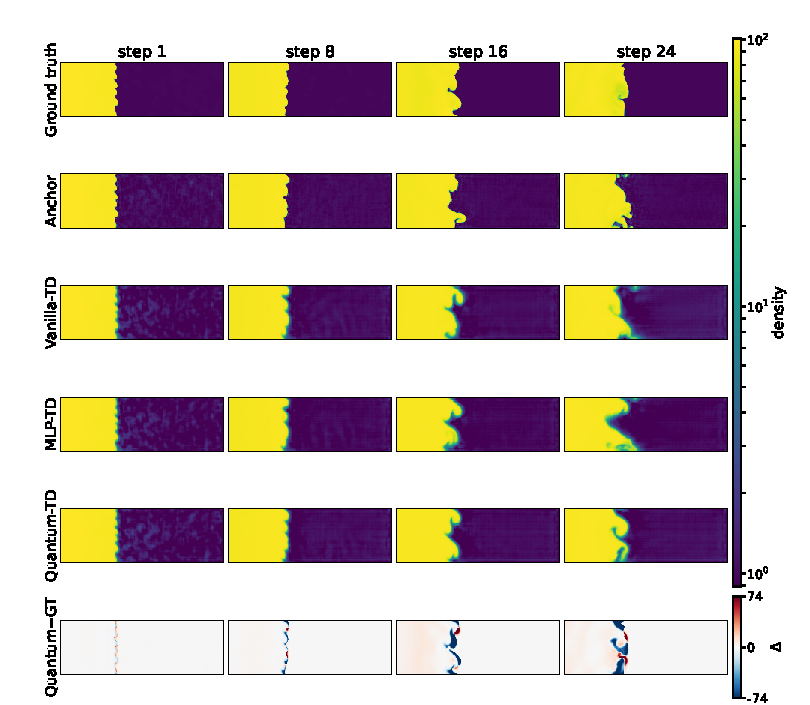
\includegraphics[width=0.58\linewidth]{fig_fields.pdf}}{}
\caption{\small Ground truth vs model rollouts on the first TRL2D test trajectory
(density, log scale; hardest cooling-time regime; rows: models, columns:
rollout steps; bottom: signed Quantum-TD error). Error concentrates at the
mixing front: at step 24, 83\% of Quantum-TD squared density error lies in
the top-decile $|\nabla\rho|$ band (10\% of pixels). On this one trajectory
the anchor has the lowest late-step VRMSE (0.640/0.659 at steps 16/24 vs
Quantum-TD 0.890/0.712, best TD arm) while Quantum-TD tracks the front best
(mean displacement 8.7\,px vs 17.0 vanilla, 22.1 MLP, 10.0 anchor);
headline claims rest on full-test-set averages (Table~\ref{tab:campaign}).}
\label{fig:fields}
\end{figure}

\subsection{Mechanism: inference-inert registers whose interactions matter in training}
\label{sec:mechanism}

Our dequantization suite shows the trained adapter is
\emph{inference-inert}: product-state and $\chi{=}1$ surrogates, 128-shot
readout, and even zeroing the readout reproduce the fine-tuned model's
rollout VRMSE to within $2{\times}10^{-5}$ (600$\times$ below seed noise).
The mean von Neumann entropy across the balanced $5|5$ bipartition of each
trained 10-qubit register, over validation inputs, is 0.03--0.09 bits;
that zeroing the readout changes nothing means the trained gate is
effectively closed. The quantum arm's gain therefore points to a
\emph{training-dynamics} effect --- the bottleneck steers TD fine-tuning
into a better basin that is then encoded in the trunk --- consistent with
our pre-registered framing of quantum-structured inductive bias rather than
inference-time quantum computation. Neighbors report pieces of this
pattern in other settings --- faster convergence of hybrid PINNs
\citep{klement2026qpinn}, quantum-assisted training with classical
inference by design \citep{chen2026dropprior}, and reservoirs whose
short-range entanglement is load-bearing at inference yet MPS-simulable
\citep{delorenzis2025qelm} --- but none tests both inference-inertness and
training-side interaction necessity. \AblationVerdict

\subsection{Cross-domain preliminary: MHD\_64}
\label{sec:mhd}

On The Well's 3-D, 7-channel \texttt{MHD\_64}, the released official
CNextU-net checkpoint does not reproduce its paper claim of 0.1633 under
our evaluation pipeline --- the same pipeline reproduces the TRL2D anchor
to 1.1\%, which localizes the discrepancy to the released artifact
(reported upstream): we measure $\approx$0.66 on both validation and test.
Our checkpoint-surgery fine-tunes recover it to the 0.177 level (single
seed, validation only, test untouched): at 20k steps all three arms ---
vanilla, quantum $3{\times}10$q, and matched-MLP --- reach validation VRMSE
\MHDmlp{} (undifferentiated at one seed;
Figure~\ref{fig:training}, right). This is
preliminary cross-domain evidence that the surgery pipeline transfers; no
quantum-versus-control claim is made at one seed.

\section{Limitations and future work}
\label{sec:limitations}

This is a preliminary study: three seeds per arm, one primary benchmark, a
single-seed validation-only MHD probe, an internal sprint arena whose
ladder saturates at its difficulty, and per-trajectory tests underpowered
at nine trajectories. All quantum components are classically simulated; at
$\le$30 qubits every claim is an inductive-bias claim, not a
quantum-advantage claim \citep{schuld2022advantage,cerezo2025barren}, the
stance is utilitarian, and the trunk sees only $n$ linear readouts per
register. Every experiment, including each negative result, runs on one
121\,GiB workstation and regenerates from one command per table.

\paragraph{Positions on the workshop's open questions.}
\emph{(1)~Correctness:} physical consistency over official rollout windows
against the spatial-mean floor, paired per-window tests, pre-registered
kill rules, and diagnosis of where error lives (Fig.~\ref{fig:fields}) ---
not pixel fidelity alone. \emph{(2)~Pixels vs.\ latents:} the surrogate
predicts in observation space (inspectable rollouts) while the register
acts on a pooled latent and returns $n$ readouts, an identifiable
low-dimensional latent by construction. \emph{(3)~Long horizons:} the only
gain appears on the hardest horizon window and only under rollout-aware
training; action-controllability is untested. \emph{(4)~Sim-to-real:} the
simulation-trained surrogate still degrades past the spatial-mean floor at
long horizons, so it augments rather than replaces the solver; device
mapping of the register is untested. \emph{(5)~Scaling laws:} accuracy
versus qubit count is flat from five qubits at this difficulty; the
question must be posed on harder analog cores.

\paragraph{Future work.} (i)~\emph{Power:} the full $3{\times}3$ MHD grid,
more seeds and trajectories. (ii)~\emph{Mechanism:} the official-protocol Gutzwiller arms and an entanglement-versus-gain correlation. (iii)~\emph{Harder analog cores:} the ladder, extended above
30 qubits by register count and size, on 3-D MHD, frozen video world
models scored by physics judges
\citep{gao2026lingbotworld,wan2025wan,motamed2025physicsiq,li2025worldmodelbench},
and industrial energy surrogates (tokamak transport and magnetics,
equilibrium reconstruction, geothermal plumes). (iv)~\emph{Configuration
search:} an evolved register bank with routing, reinforcement-learning and
quantum-architecture-search over parameterized register graphs
\citep{zoph2017neural,du2022quantum}, and temporal-difference test-time
adaptation. (v)~\emph{Hardware:} device-constraint mapping, emulator fidelity, small hardware micro-runs.

\bibliographystyle{plainnat}
\bibliography{references}

\end{document}
